\section{Correction des exercices}

\frame
{
    \frametitle{Exercice 1}
	\begin{block}{\'Enonc\'e}
		Trouver l'ensemble des attributs obligatoires pour une IRM.
	\end{block}
}

\frame
{
    \frametitle{Exercice 2}
    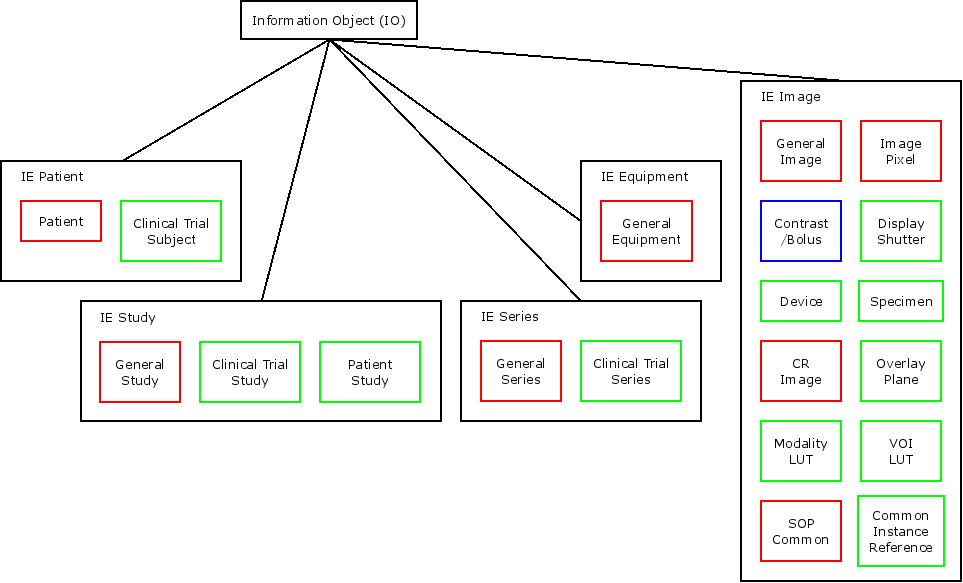
\includegraphics[width=\linewidth]{./figures/IO-definition-IE.png}

}

\frame
{
    \frametitle{Exercice 3}

    \begin{block}{Exercice}
        Jusqu'\`a combien pouvez-vous compter avec vos $10$ doigts ?
    \end{block}

    \begin{block}{R\'eponse}
        1023
    \end{block}

    \begin{center}
        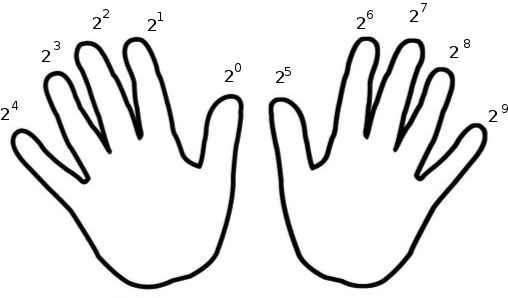
\includegraphics[width=.5\linewidth]{./figures/digits.png}
    \end{center}

}

